% la-04-vectors.tex

\documentclass[xcolor=dvipsnames]{beamer}
\usepackage{teachbeamer}

\title{Vectors}
\subtitle{{\CourseNumber}, BCIT}

\author{\CourseName}

\date{October 1, 2018}

\begin{document}

\begin{frame}
  \titlepage
\end{frame}

\begin{frame}
  \frametitle{Vectors}
  A vector space $V$ over a field $F$ is a set on which two operations
  (addition and scalar multiplication) are defined. Some axioms need
  to be fulfilled, most relevantly \alert{closure} with respect to
  addition and scalar multiplication:
  \begin{itemize}
  \item If $v,w\in{}V$, then $v+w\in{}V$
  \item If $a\in{}F,v\in{}V$, then $av\in{}V$
  \end{itemize}
  In this course, the field will always be $\mathbb{R}$ or
  $\mathbb{C}$, the real or the complex numbers.
\end{frame}

\begin{frame}
  \frametitle{Linear Combination and Span}
  If $T=\{v_{1},{\ldots},v_{k}\}$ is a set of vectors and
  $\{x_{1},{\ldots},x_{k}\}\subset{}F$ is a set of scalars, then
  \begin{equation}
    \label{eq:aiveatah}
    x_{1}v_{1}+{\ldots}+x_{k}v_{k}
  \end{equation}
  is called a \alert{linear combination} of $v_{1},{\ldots},v_{k}$.
  The set of all linear combinations of $v_{1},{\ldots},v_{k}$ is
  called the \alert{span} of $v_{1},{\ldots},v_{k}$.

  \medskip

  The span of a set of vectors is a \alert{subspace} of $V$, meaning
  that it is closed with respect to addition and scalar
  multiplication. The solution set for a system of linear equations is
  always a subspace (if $u,v\in{}S$ and $a\in{}F$, then $u+v\in{}S$
  and $au\in{}S$).
\end{frame}

\begin{frame}
  \frametitle{Linear Independence}
  A set of vectors $v_{1},{\ldots},v_{k}$ is \alert{linearly
    independent} if and only if the vector equation
  \begin{equation}
    \label{eq:wohsiete}
    x_{1}v_{1}+{\ldots}+x_{k}v_{k}=0    
  \end{equation}
  has the unique solution $(x_{1},{\ldots},x_{k})=(0,{\ldots},0)$.
\end{frame}

\begin{frame}
  \frametitle{Theorems of Linear Independence}
  \begin{enumerate}
  \item $v_{1},{\ldots},v_{k}$ are linearly dependent if and only if
    at least one of these vectors is a linear combination of the
    others
  \item The columns of a matrix $A$ are linearly independent if and
    only if the rank of $A$ is $k$ (the number of columns).
  \item A square matrix is invertible if and only if its columns (or
    rows) are linearly independent.
  \end{enumerate}
\end{frame}

\begin{frame}
  \frametitle{Basis and Dimension}
  If $V$ is a vector space, then the set $B=\{b_{1},{\ldots},b_{k}\}$
  is a \alert{basis} of $V$ if and only if $v_{1},{\ldots},v_{k}$ are linearly
  independent and the span of $B$ is $V$.
  \begin{block}{Unique Representation}
    Every vector $u\in{}V$ is a linear combination
    $u=x_{1}b_{1}+{\ldots}+x_{k}b_{k}$ of basis vectors, if such a basis
    exists. The ordered set $(x_{1},{\ldots},x_{k})$ is called the
    \alert{coordinates} of $u$ with respect to basis $B$. 
  \end{block}
  There is a theorem that tells us that if two sets of vectors $B_{1}$
  and $B_{2}$ are bases of vector space $V$, then the cardinality of
  $B_{1}$ equals the cardinality of $B_{2}$. Thus, if a finite base
  exists, it makes sense to define the \alert{dimension} of the vector
  space to be the cardinality of that base.
\end{frame}

\begin{frame}
  \frametitle{Vector Spaces}
  A finite-dimensional vector space (let the dimension be $n$) over
  the real numbers corresponds to a set of ordered sets of real
  numbers (the coordinates of the vectors). In other words, it
  corresponds to $\mathbb{R}^{n}$. 

\medskip

Examples of vector spaces:
\begin{itemize}
\item three-dimensional space $\mathbb{R}^{3}$
\item the set of all straight lines in two-dimensional space
\item the set of all parabolas in two-dimensional space
\item the set of all circles in two-dimensional space
\item the set of all polynomials with degree $k\leq{}n$
\item the set of all real-valued functions on $\mathbb{R}$
\end{itemize}
Try to determine the dimensions of these vector spaces.
\end{frame}

\begin{frame}
  \frametitle{Displacement Vectors}
  One way to interpret a vector in $\mathbb{R}^{2}$ or
  $\mathbb{R}^{3}$ is to make it refer to a point in the
  $xy$-plane or $xyz$-three-dimensional space. The usual
  interpretation, however, is as a \alert{displacement vector} with a
  direction and a length. Here is an example:
  \begin{equation}
    \label{eq:lapheeka}
    \vec{v}=\left(
    \begin{array}{c}
      3 \\
      5 \\
      -1
    \end{array}\right)
  \end{equation}
\end{frame}

\begin{frame}
  \frametitle{Vector Algebra}
  Vectors can be added, subtracted, and multiplied by a scalar (a real
  number).
  \begin{equation}
    \label{eq:kaepuema}
    \left(
    \begin{array}{c}
      3 \\
      5 \\
      -1
    \end{array}\right)+
  \left(
    \begin{array}{c}
      2 \\
      \pi \\
      -6
    \end{array}\right)=
  \left(
    \begin{array}{c}
      5 \\
      5+\pi \\
      -7
    \end{array}\right)
  \end{equation}
  \begin{equation}
    \label{eq:kemodaim}
    1.5\cdot\left(
    \begin{array}{c}
      3 \\
      5 \\
      -1
    \end{array}\right)=
  \left(
    \begin{array}{c}
      4.5 \\
      7.5 \\
      -1.5
    \end{array}\right)
  \end{equation}
\end{frame}

\begin{frame}
  \frametitle{Length and Angle of Vector}
  Two-dimensional and three-dimensional vectors in $\mathbb{R}^{2}$
  and $\mathbb{R}^{3}$ are easily visualized. They have a length and a
  direction (in two-dimensional space, the direction can be
  represented by an angle). We use the dot product to define length
  and angle for any vectors. Let $V$ be an $n$-dimensional vector
  space with a basis. Let $u$ and $v$ be vectors whose coordinates
  with respect to the basis are $(u_{1},{\ldots},u_{n})$ and
  $(v_{1},{\ldots},v_{n})$. Organize the coordinate vectors as
  one-column matrices $\vec{u}$ and $\vec{v}$. Then the dot product is
  defined using matrix multiplication.
  \begin{equation}
    \label{eq:emiehoij}
    u\cdot{}v=\vec{u}\,^{\intercal}\cdot\vec{v}
  \end{equation}
\end{frame}

\begin{frame}
  \frametitle{Length and Angle of Vector}
  Now verify that in the two-dimensional case, the length of a vector $u$
  is
  \begin{equation}
    \label{eq:zuabiemu}
    \Vert{}u\Vert^{2}=u\cdot{}u
  \end{equation}
  and its angle is
  \begin{equation}
    \label{eq:iechaigu}
    \cos\theta=\frac{u\cdot{}v}{\Vert{}u\Vert\cdot\Vert{}v\Vert}
  \end{equation}
  For vectors not in $\mathbb{R}^{2}$, let length and angle be so
  defined. Two vectors $u$ and $v$ are \alert{perpendicular}, or
  \alert{orthogonal}, if and only if $v\cdot{}w=0$.
\end{frame}

% \begin{frame}
%   \frametitle{Unit Vectors}
%   All three-dimensional vectors can be expressed in components. For
%   this expression we need unit vectors. Any three linearly independent
%   vectors would work, but it makes sense to use the following three:
%   \begin{equation}
%     \label{eq:bahniech}
%     \vec{i}=\left(
%     \begin{array}{c}
%       1 \\
%       0 \\
%       0
%     \end{array}\right)\hspace{.2in}
%     \vec{j}=\left(
%     \begin{array}{c}
%       0 \\
%       1 \\
%       0
%     \end{array}\right)\hspace{.2in}
%     \vec{k}=\left(
%     \begin{array}{c}
%       0 \\
%       0 \\
%       1
%     \end{array}\right)
%   \end{equation}
% \end{frame}

% \begin{frame}
%   \frametitle{Vector Decomposition}
%   For any vector $\vec{v}$  (assuming from now on three dimensions),
%   \begin{equation}
%     \label{eq:teequahg}
%     \vec{v}=v_{x}\vec{i}+v_{y}\vec{j}+v_{z}\vec{k}
%   \end{equation}
% where $V=(v_{x},v_{y},v_{z})$, and $V$ is the point to which the
% origin $O=(0,0,0)$ would be displaced by vector
% \begin{equation}
%   \label{eq:zaegiexo}
%   \vec{v}=\left(
%     \begin{array}{c}
%       v_{x} \\
%       v_{y} \\
%       v_{z} \\
%     \end{array}\right)
% \end{equation}
% \end{frame}

% \begin{frame}
%   \frametitle{Vector Length and Distance Between Two Points}
%   The length of vector $\vec{v}$ is
%   \begin{equation}
%     \label{eq:ogeithie}
%     \Vert\vec{v}\Vert=\sqrt{v_{x}^{2}+v_{y}^{2}+v_{z}^{2}}
%   \end{equation}
% The distance between two points $P$ and $Q$ is the length of a
% displacement vector between them. Let $\vec{OP}$ be the displacement
% vector from $O$ to $P$ and so on. Then
% \begin{equation}
%   \label{eq:ahnoocae}
%   \vec{PQ}=\vec{PO}+\vec{OQ}=\vec{OQ}-\vec{OP}
% \end{equation}
% and $\Vert\vec{PQ}\Vert$ is the distance between $P$ and $Q$.
% \end{frame}

\begin{frame}
  \frametitle{Dot Product}
  The following two definition of the \alert{dot product}, or
  \alert{scalar product}, $\vec{v}\cdot\vec{w}$ are equivalent:
  \begin{description}
  \item[geometric]
    $\vec{v}\cdot\vec{w}=\Vert\vec{v}\Vert\cdot\Vert\vec{w}\Vert\cdot\cos\vartheta$
    where $\vartheta$ is the angle between $\vec{v}$ and $\vec{w}$,
    $0\leq\vartheta\leq\pi$.
  \item[algebraic] $\vec{v}\cdot\vec{w}=v_{x}w_{x}+v_{y}w_{y}+v_{z}w_{z}$
  \end{description}
The dot product is a number, not a vector.
\end{frame}

\begin{frame}
  \frametitle{Dot Product}
  Now we need to show that the two definitions are equivalent.
  Consider a triangle $PQR$ in three-dimensional space. Let
  $\vec{v}=\vec{PQ},\vec{w}=\vec{PR}$. Then
  \begin{equation}
    \label{eq:oobeipho}
  \vec{QR}=\vec{QP}+\vec{PR}=-\vec{v}+\vec{w}=\vec{w}-\vec{v}  
\end{equation}
Here is the law of cosines for this triangle:
\begin{equation}
  \label{eq:aiwahzoa}
  \Vert\vec{w}-\vec{v}\Vert^{2}=\Vert\vec{v}\Vert^{2}+\Vert\vec{w}\Vert^{2}-2\Vert\vec{v}\Vert\cdot\Vert\vec{w}\Vert\cos\vartheta
\end{equation}
It follows that the two definitions are equivalent.
\end{frame}

% \begin{frame}
%   \frametitle{Dot Product}
% \begin{block}{Perpendicularity and Dot Product}
%   Two non-zero vectors $\vec{v}$ and $\vec{w}$ are perpendicular, or
%   orthogonal, if and only if $\vec{v}\cdot\vec{w}=0$.
% \end{block}

% \bigskip

% \begin{block}{Magnitude and Dot Product}
%   Magnitude and dot product are related as follows: $\vec{v}\cdot\vec{v}=\Vert\vec{v}\Vert$.
% \end{block}
% \end{frame}

% this is NOT correct
% \begin{frame}
%   \frametitle{Dot Product Exercise}
%   {\ubung} Find a normal vector to the following planes (a normal vector to a
%   plane is perpendicular to all non-zero vectors displacing points on
%   the plane).
%   \begin{equation}
%     \label{eq:afanaagu}
%     2x+y-z=5
%   \end{equation}
%   \begin{equation}
%     \label{eq:reeregha}
%     2(x-z)=3(x+y)
%   \end{equation}
%   For (\ref{eq:afanaagu}), set $x=1,y=1$, then $z=-2$ for
%   $P=(1,1,-2)$. Then set $x=3,y=1$, so $z=2$ for $Q=(3,1,2)$. Both $P$
%   and $Q$ are on the plane, so $\vec{PQ}=\vec{OQ}-\vec{OP}$ is a
%   vector displacing two points in the plane. To find a vector
%   perpendicular to it consider the dot product
% \begin{equation}
%   \label{eq:chiemaig}
%   -2x+0y-4z=0
% \end{equation}
% Choose $x=1,y=1$, so $z=-0.5$. The vector
% $1\cdot\vec{i}+1\cdot\vec{j}-0.5\cdot\vec{k}$ is a normal vector to the
% plane $2x+y-z=5$.
% \end{frame}

\begin{frame}
  \frametitle{Dot Product Exercise}
  {\ubung} Find the angle between
  \begin{equation}
    \label{eq:tauhohju}
    \vec{v}=\left(
      \begin{array}{c}
        4 \\
        0 \\
        7
      \end{array}\right)\hspace{.5in}\vec{w}=\left(
      \begin{array}{c}
        -2 \\
        1 \\
        3
      \end{array}\right)
  \end{equation}
  Consider the dot product
  \begin{equation}
    \label{eq:ijaquahd}
    4\cdot(-2)+0\cdot{}1+7\cdot{}3=13
  \end{equation}
According to the two equivalent definitions of the dot product, this
is equal to
\begin{equation}
  \label{eq:ohyizaeb}
  \Vert\vec{v}\Vert\cdot\Vert\vec{w}\Vert\cdot\cos\vartheta=\sqrt{4^{2}+7^{2}}\cdot\sqrt{(-2)^{2}+1^{2}+3^{2}}\cdot\cos\vartheta
\end{equation}
Therefore,
\begin{equation}
  \label{eq:yohsheen}
  \vartheta=\arccos\frac{13}{\sqrt{4^{2}+7^{2}}\cdot\sqrt{(-2)^{2}+1^{2}+3^{2}}}=64.47^{\circ}
\end{equation}
\end{frame}

\begin{frame}
  \frametitle{Planes Again}
  The equation of the plane with normal vector
  $\vec{n}=a\vec{i}+b\vec{j}+c\vec{k}$ and containing the point
  $P=(x_{0},y_{0},z_{0})$ is
  \begin{equation}
    \label{eq:ijaeriri}
    a(x-x_{0})+b(y-y_{0})+c(z-z_{0})=0
  \end{equation}
  Alternatively, for $d=ax_{0}+by_{0}+cz_{0}$
  \begin{equation}
    \label{eq:bamoyeez}
    ax+by+cz=d
  \end{equation}
\end{frame}

\begin{frame}
  \frametitle{Orthonormal Basis}
  If a basis consists of vectors which are
  \begin{enumerate}
  \item pairwise orthogonal and
  \item all have length 1
  \end{enumerate}
  then the basis is an \alert{orthonormal basis}. A vector $w$ can always
  be scaled to length 1 by multiplying it by $1/\Vert{}w\Vert$.

  \medskip

  An orthogonal matrix $Q$ consists of columns which form an orthonormal
  basis. It can be shown that $Q^{\intercal}Q=Q^{\intercal}Q=I$,
  therefore $Q^{\intercal}=Q^{-1}$. 
\end{frame}

\begin{frame}
  \frametitle{Orthonormal Basis Exercise}
% Paul C. Shields, page 227
  {\ubung} Find an orthonormal basis for the plane whose equation is
  \begin{equation}
    \label{eq:deidongo}
    2x-3y+7z=0
  \end{equation}
\end{frame}

\begin{frame}
  \frametitle{QR Matrix Factorization}
  There are several matrix factorization theorems. For example, if you
  order the rows and columns of a square matrix $A$ intelligently,
  then $A=LU$, where $L$ is a lower triangular matrix and $U$ is an
  upper triangular matrix. Computers use this factorization to find
  determinants and solutions for systems of linear equations.
  \begin{block}{QR Factorization Theorem}
    Any real square matrix $A$ can be decomposed as $A=QR$, where $Q$
    is an orthogonal matrix and $R$ is an upper triangular matrix.
  \end{block}
  The QR factorization theorem can also be used to solve a system of
  linear equations efficiently. Assume you have a QR factorization
  machine. How would you find the solutions for a system of linear
  equations?
\end{frame}

\begin{frame}
  \frametitle{An Infinite-Dimensional Vector Space}
  Consider the set $\mathcal{F}=\{f|f\mbox{ is a continuous function
    on }\mathbb{R}\}$. Define addition by $(f+g)(x)=f(x)+g(x)$ and
  scalar multiplication by $(af)(x)=af(x)$. Then the set $\mathcal{F}$
  fulfills all the axioms for a vector space. Now define the dot
  product
  \begin{equation}
    \label{eq:ivaichoh}
    f\cdot{}g=\int_{0}^{1}f(x)g(x)\,dx
  \end{equation}
Show that $f(x)=\sin\pi{}x$ and $g(x)=\sin{}2\pi{}x$ are orthogonal to
each other. As it turns out,
$\{1,\sin{}2\pi{}x,\cos{}2\pi{}x,\sin{}4\pi{}x,\cos{}4\pi{}x,{\ldots}\}$
is a basis of orthogonal vectors for $\mathcal{F}$. Therefore, the
dimension of $\mathcal{F}$ is infinite. 
\end{frame}

\begin{frame}
  \frametitle{Tangent Planes}
  Assuming $f$ is differentiable at $(a,b)$, the equation of the
  tangent plane is
  \begin{equation}
    \label{eq:aoseenai}
z=f(a,b)+f_{x}(a,b)(x-a)+f_{y}(a,b)(y-b)
  \end{equation}
  $f(x,y)$ can be approximated around $(a,b)$ by the tangent plane,
  \begin{equation}
    \label{eq:xabixaic}
    f(x,y)\approx{}f(a,b)+\frac{\partial{}f}{\partial{}x}(a,b)(x-a)+\frac{\partial{}f}{\partial{}y}(a,b)(y-b)\mbox{ near }(a,b)
  \end{equation}
\end{frame}

\begin{frame}
  \frametitle{Tangent Planes Exercise}
  {\ubung} Find the equation of the tangent plane with respect to the
  unit circle at $P=(0.2,0.3,\sqrt{0.87})$.

  \medskip

  Hint: identify a vector that is orthogonal to the plane or use
  partial derivatives for the function whose function graph overlaps
  with the relevant part of the sphere.
\end{frame}

\begin{frame}
  \frametitle{Subspaces and Hyperplanes}
  Let $V$ be a vector space with a subset $U\subset{}V$. $U$ is a
  \alert{subspace} of $V$ if and only if $U$ is also a vector space. A
  two-dimensional plane is a subspace of three-dimensional space.
  Distinguish, however, between sets of points and sets of vectors.
  The origin is not an element of all planes in $\mathbb{R}^{3}$, but
  the zero-vector is.
\end{frame}

\begin{frame}
  \frametitle{Subspaces and Hyperplanes}
  Let $V$ be an $n$-dimensional (therefore finite-dimensional) vector
  space with a subset $H\subset{}V$. Then $H$ is a \alert{hyperplane}
  in $V$ if and only if $H$ has a basis (all and only elements of $H$
  are a linear combination of a set of basis vectors in $H$). Lines
  and planes are hyperplanes. It is relatively easy to show that in
  the finite-dimensional case, all and only hyperplanes in $V$ are
  subspaces of $V$.
\end{frame}

\begin{frame}
  \frametitle{Subspaces and Hyperplanes}
  The solution to a system of linear equations is always a hyperplane
  (of points, not of vectors) unless there is a unique solution. The
  reason is that whenever there are two distinct solutions $\vec{OP}$
  and $\vec{OQ}$, any combination $\vec{OP}+s_{1}\vec{PQ}$ with
  $s_{1}\in\mathbb{R}$ will also be a solution. Note that the empty
  set is a hyperplane.
\end{frame}

\begin{frame}
  \frametitle{Subspaces and Hyperplanes}
  \beispiel{Solving a Dependent System of Equations}
  \begin{equation}
    \label{eq:leizaewu}
    \begin{array}{ccccccc}
      3x&+&y&-&5z&=&-4 \\
      4x&+&2y&-&z&=&-5 \\
      6x&+&4y&+&7z&=&-7 \\
    \end{array}
  \end{equation}
  \textbf{Step 1.} Find the determinant of the coefficient matrix.
  \begin{equation}
    \label{eq:faiquuko}
    \det\left(\left[
        \begin{array}{ccc}
          3&1&-5 \\
           4&2&-1 \\
           6&4&7
        \end{array}\right]\right)=0
  \end{equation}
\end{frame}

\begin{frame}
  \frametitle{Subspaces and Hyperplanes}
  \textbf{Step 2.} The coefficient matrix is singular. Find the
  echelon form of the augmented matrix.
  \begin{equation}
    \label{eq:ooroosuw}
    \left[
      \begin{array}{cccc}
      1&1&4&-1 \\
      0&2&17&1 \\
      0&0&0&0
    \end{array}\right]
  \end{equation}
  The system is consistent with infinitely many solutions.

\medskip

  \textbf{Step 3.} From the second row, we learn that
\begin{equation}
  \label{eq:ahpoquah}
  y=\frac{1}{2}-\frac{17}{2}z
\end{equation}
Plug this into the first row for
\begin{equation}
  \label{eq:zayochee}
  x=-\frac{3}{2}-\frac{25}{2}z
\end{equation}
One solution is $(3,-8,1)$. Another is $(-\frac{3}{2},\frac{1}{2},0)$. 
\end{frame}

\begin{frame}
  \frametitle{Subspaces and Hyperplanes}
  \textbf{Step 4.} $z$ is here a free variable. Once the free
  variables are arbitrarily fixed, the other variables are determined
  as well. The solution space in this case is one-dimensional (a line
  in three-dimensional space). For an $n$-dimensional solution space
  and a solution $v_{0}$, express the solution space as a linear
  combination of its basis vectors $v_{1},{\ldots},v_{n}$ (make sure
  they are linearly independent).
  \begin{equation}
    \label{eq:geeduboh}
    S=\left\{v_{0}+s_{1}v_{1}+{\ldots}+s_{n}v_{n}|s_{1},{\ldots},s_{n}\in\mathbb{R}\right\}
  \end{equation}
  \begin{equation}
    \label{eq:shoxuqui}
    S=\left.\left\{\left(
        \begin{array}{c}
          3 \\
          -8 \\
          1
        \end{array}\right)+s_{1}\left(
        \begin{array}{c}
          -9 \\
          17 \\
          -2
        \end{array}\right)\right\vert{}s_{1}\in\mathbb{R}\right\}
  \end{equation}
\end{frame}

\begin{frame}
  \frametitle{Subspaces and Hyperplanes}
  {\ubung} Solve the following system of linear equations:
  \begin{equation}
    \label{eq:xohvaesh}
    \begin{array}{ccccccccc}
      4x_{1}&+&x_{2}&+&5x_{3}&-&7x_{4}&=&14 \\
      -3x_{1}&+&5x_{2}&-&x_{3}&-&2x_{4}&=&-18 \\
      11x_{1}&-&3x_{2}&+&11x_{3}&-&12x_{4}&=&46 \\
      10x_{1}&-&9x_{2}&+&7x_{3}&-&3x_{4}&=&50
    \end{array}
  \end{equation}
\end{frame}

\begin{frame}
  \frametitle{Subspaces and Hyperplanes}
  Solution: create the coefficient matrix and calculate the
  determinant.
  \begin{equation}
    \label{eq:pepheiwo}
    \left\vert
      \begin{array}{cccc}
        4&1&5&-7 \\
         -3&5&-1&-2 \\
         11&-3&11&-12 \\
         10&-9&7&-3
      \end{array}\right\vert=0
  \end{equation}
\end{frame}

\begin{frame}
  \frametitle{Subspaces and Hyperplanes}
The determinant is zero, therefore there are dependent equations. Find
the echelon form of the augmented matrix.
\begin{equation}
  \label{eq:iaphuuth}
  \left[
    \begin{array}{ccccc}
1 & 6 & 4 & -9 & -4 \\
0 & 23 & 11 & -29 & -30 \\
0 & 0 & 0 & 0 & 0 \\
0 & 0 & 0 & 0 & 0 
    \end{array}\right]
\end{equation}
The system is consistent with infinitely many solutions, and there are
two free variables. The solution space is a two-dimensional hyperplane
in four-dimensional space. 
\end{frame}

\begin{frame}
  \frametitle{Subspaces and Hyperplanes}
  Find three linearly independent solutions.
  \begin{enumerate}
  \item If $x_{4}=1,x_{3}=2$, then the top two rows of the echelon
    form determine $x_{2}=-1,x_{1}=3$.
  \item If $x_{4}=0,x_{3}=0$, then the top two rows of the echelon
    form determine $x_{2}=-\frac{30}{23},x_{1}=\frac{88}{23}$.
  \item If $x_{4}=1,x_{3}=-1$, then the top two rows of the echelon
    form determine $x_{2}=\frac{10}{23},x_{1}=\frac{147}{23}$.
  \end{enumerate}
  Consequently,
  \begin{equation}
    \label{eq:eidichee}
    S=\left\{\left.\left(
        \begin{array}{c}
          3 \\
          -1 \\
          2 \\
          1
        \end{array}\right)+s_{1}\left(
        \begin{array}{c}
          19 \\
          -7 \\
          -46 \\
          -23
        \end{array}\right)+s_{2}\left(
        \begin{array}{c}
          78 \\
          33 \\
          -69 \\
          0
        \end{array}\right)\right\vert{}s_{1},s_{2}\in\mathbb{R}\right\}
  \end{equation}
\end{frame}

\begin{frame}
  \frametitle{Cross Product}
  \begin{figure}[h]
    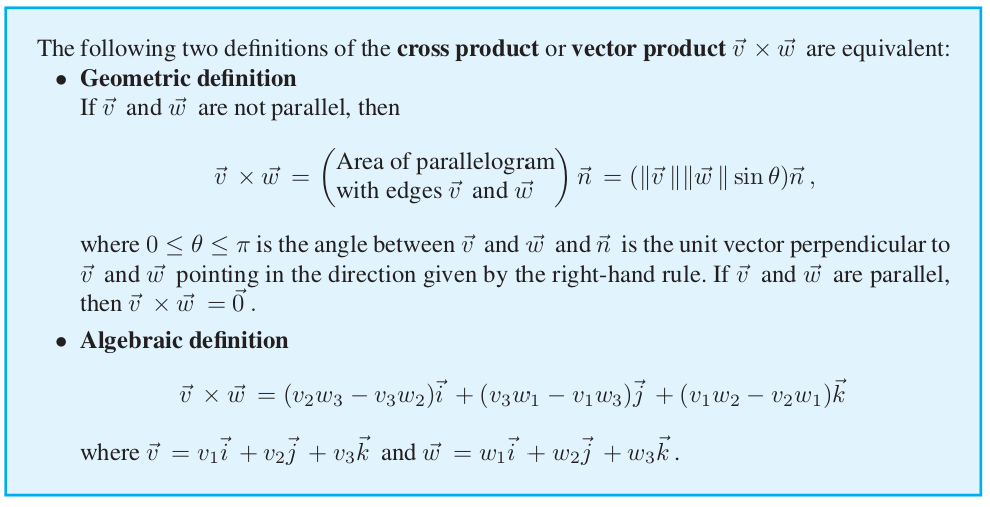
\includegraphics[scale=0.32]{./diagrams/crossproduct.png}
  \end{figure}
\end{frame}

\begin{frame}
  \frametitle{Cross Product}
  If you know what a determinant is, you can remember the algebraic
  definition as follows.
  \begin{equation}
    \label{eq:abeekohc}
    \vec{v}\times\vec{w}=\left\vert
      \begin{array}{ccc}
        \vec{i} & \vec{j} & \vec{k} \\
        v_{1} & v_{2} & v_{3} \\
        w_{1} & w_{2} & w_{3}
      \end{array}\right\vert
  \end{equation}
  Note that $\vec{w}\times\vec{v}=-\vec{v}\times\vec{w}$.
\end{frame}

\begin{frame}
  \frametitle{Cross Product Exercise}
% Paul C. Shields, page 264, sol 1/(3*sqrt(46))*(-7,-19,2)
  {\ubung} Find a unit vector that is perpendicular to both
  $\vec{u}=(3,-1,1)^{\intercal}$ and $\vec{v}=(2,0,7)^{\intercal}$
\end{frame}

\begin{frame}
  \frametitle{Cross Product Exercise}
  {\ubung} Use the cross product to find the linear equation containing the
  three points
  \begin{equation}
    \label{eq:eiyeigaz}
    \begin{array}{rcl}
      P&=&(1,3,0) \\
      Q&=&(3,4,-3) \\
      R&=&(3,6,2)
    \end{array}
  \end{equation}
\end{frame}

\begin{frame}
  \frametitle{Cross Product Exercise Answer}
One way to find the answer to the last exercise (without using the
cross product) is to solve the following system of linear equations
for the plane $x+ay+bz=c$,
\begin{equation}
  \label{eq:yohghaef}
  \begin{array}{rcl}
    1+3a+0b&=&c \\
    3+4a-3b&=&c \\
    3+6a+2b&=&c
  \end{array}
\end{equation}
Change this to
\begin{equation}
  \label{eq:oxeingiu}
  \begin{array}{rcl}
    3a+0b-c&=&-1 \\
    4a-3b-c&=&-3 \\
    6a+2b-c&=&-3 \\
  \end{array}
\end{equation}
Using matrices,
\begin{equation}
  \label{eq:ukohjiej}
  \left(
    \begin{array}{ccc}
      3&0&-1 \\
      4&-3&-1 \\
      6&2&-1
    \end{array}\right)\cdot\left(
    \begin{array}{c}
      a \\
      b \\
      c
    \end{array}\right)=\left(
    \begin{array}{c}
      -1 \\
      -3 \\
      -3
    \end{array}\right)
\end{equation}
\end{frame}

\begin{frame}
  \frametitle{Cross Product Exercise Answer}
  Equation (\ref{eq:ukohjiej}) yields the solution
  \begin{equation}
    \label{eq:maeshael}
      x-\frac{10}{11}y+\frac{4}{11}z=-\frac{19}{11}
  \end{equation}
Now let's use the cross product instead, avoiding the matrices. Note
that
\begin{equation}
  \label{eq:ushahroh}
  \begin{array}{rcl}
    \vec{PQ}&=&2\vec{i}+\vec{j}-3\vec{k} \\
    \vec{PR}&=&2\vec{i}+3\vec{j}+2\vec{k}
  \end{array}
\end{equation}
The cross product, using the algebraic definition, is
$\vec{u}=\vec{PQ}\times\vec{PR}=11\vec{i}-10\vec{j}+4\vec{k}$.
\end{frame}

\begin{frame}
  \frametitle{Cross Product Exercise Answer}
  Let $P=(x_{0},y_{0},z_{0})$ be a fixed point on the plane with known
  coordinates. Since any point $S=(x,y,z)$ on the plane fulfills
\begin{equation}
  \label{eq:iefeeboh}
  \vec{PS}\cdot\vec{u}=0
\end{equation}
this can be turned into the plane equation
\begin{equation}
  \label{eq:vetiexup}
  u_{x}(x-x_{0})+u_{y}(y-y_{0})+u_{z}(z-z_{0})=0
\end{equation}
Therefore, using $P=(1,3,0)$, this translates into
\begin{equation}
  \label{eq:eechawoi}
11x-10y+4z=19  
\end{equation}
which is equivalent to (\ref{eq:maeshael}). Notice how easy it is to
find a linear equation when you have a point $P=(x_{0},y_{0},z_{0})$
on the plane and a normal vector $\vec{u}$ to the plane
$u_{x}\vec{i}+u_{y}\vec{j}+u_{z}\vec{k}$:
\begin{equation}
  \label{eq:quaghoob}
u_{x}x+u_{y}y+u_{z}z=u_{x}x_{0}+u_{y}y_{0}+u_{z}z_{0}
\end{equation}
\end{frame}

\begin{frame}
  \frametitle{Exercise}
  {\ubung} Find all interior angles for and the plane equation
  containing the triangle with points
  \begin{equation}
    \label{eq:yeibieba}
    P=(1,4,-2),Q=(-1,1,2),R=(-1,3,1)
  \end{equation}
\end{frame}

\begin{frame}
  \frametitle{End of Lesson}
Next Lesson: Least Squares Approximation
\end{frame}

\end{document}

